\documentclass[dvipdfmx]{jsarticle}
\usepackage[T1]{fontenc}
\usepackage[dvipdfmx]{hyperref}
\usepackage{lmodern}
\usepackage{latexsym}
\usepackage{amsfonts}
\usepackage{amssymb}
\usepackage{mathtools}
\usepackage{nccmath}
\usepackage{amsthm}
\usepackage{multirow}
\usepackage[dvipdfmx]{graphicx}
\usepackage{wrapfig}
\usepackage{here}
\usepackage{float}
\usepackage{ascmac}
\usepackage{url}

\def\NO{03}
\def\LECTURENAME{論理と計算}
\begin{document}
\title{\LECTURENAME{}:第\NO{}回演習問題}

\author{5419045 高林秀}

\date{}
\maketitle

\begin{itemize}
\item Latexを用いて作成し,PDF形式で提出してください
\end{itemize}


\vspace*{\baselineskip}

\begin{enumerate}\setlength{\itemsep}{\baselineskip}
\item 推論手続き($\vdash$)の観点から伴意関係($\models$)との関係を説明しなさい.
\paragraph{解答}\par
推論手続きにおいては、得られた結果が正しいものでなくてはいけない健全性と、得られるすべての結果を漏らすことなく正しい結果を得なくてはならない完全性の2つの性質を満たすことが求められる。その上で伴意関係はトートロジーであるかどうかを確認知ればよい。


\item 次の命題文をそれぞれ節形式(=連言標準形)に変換しなさい.
  \begin{itemize}
  \item $(a\land b)\Leftrightarrow c$
  \paragraph{解答}\par
  同値記号の定義より、
  \begin{align*}
    ((a \wedge b) \Rightarrow c) \wedge (c \Rightarrow(a\wedge b)) \\
  \end{align*}
  含意記号の定義より、
  \begin{align*}
    (\neg (a \wedge b) \vee c) \wedge (\neg c \vee (a \wedge b))
  \end{align*}
  選言の交換率より、
  \begin{align*}
    (c \vee \neg(a \wedge b)) \wedge (\neg c \vee (a \wedge b))
  \end{align*}
  ド・モルガンの法則より、
  \begin{align*}
    (c \vee \neg a \vee \neg b) \wedge (\neg c \vee (a \wedge b))
  \end{align*}
  分配率より、
  \begin{align*}
    (c \vee \neg a \vee \neg b) \wedge ((\neg c \vee a)\wedge (\neg c \vee b))
  \end{align*}

  \item $(p\Rightarrow q)\Rightarrow(r\Rightarrow s)$
  \end{itemize}
  \paragraph{解答}\par
  含意文の定義より、
  \begin{align*}
    (\neg p \vee q) \Rightarrow (\neg r \vee s)
  \end{align*}
  含意文の定義より、
  \begin{align*}
    \neg(\neg p \vee q) \vee (\neg r \vee s)
  \end{align*}
  ド・モルガンの法則より、
  \begin{align*}
    (\neg \neg p \wedge \neg q) \vee (\neg r \vee s)
  \end{align*}
  二重否定から、
  \begin{align*}
    (p \wedge \neg q) \vee (\neg r \vee s)
  \end{align*}
  選言の結合律より、
  \begin{align*}
    ((p \wedge \neg q) \vee \neg r) \vee s
  \end{align*}
  選言の交換率より
  \begin{align*}
    s \vee (\neg r \vee (p \wedge \neg q))
  \end{align*}
  分配率から、
  \begin{align*}
    s \vee ((\neg r \vee p) \wedge (\neg r \vee \neg q))
  \end{align*}
  もう一度分配率を適用して、
  \begin{align*}
      (s \vee (\neg r \vee p)) \wedge (s \vee (\neg r \vee \neg q))
  \end{align*}
\item 節集合$G\,=\,\{p,\, p\Rightarrow q\}$, $r$を任意の命題記号とする.
  \begin{itemize}
  \item 真理値表を作成し,$G \models q\lor r$が成り立つことを確認しなさい.
  \paragraph{解答}\par
  真理値表は下図。
  \begin{figure}[H]
    \centering
    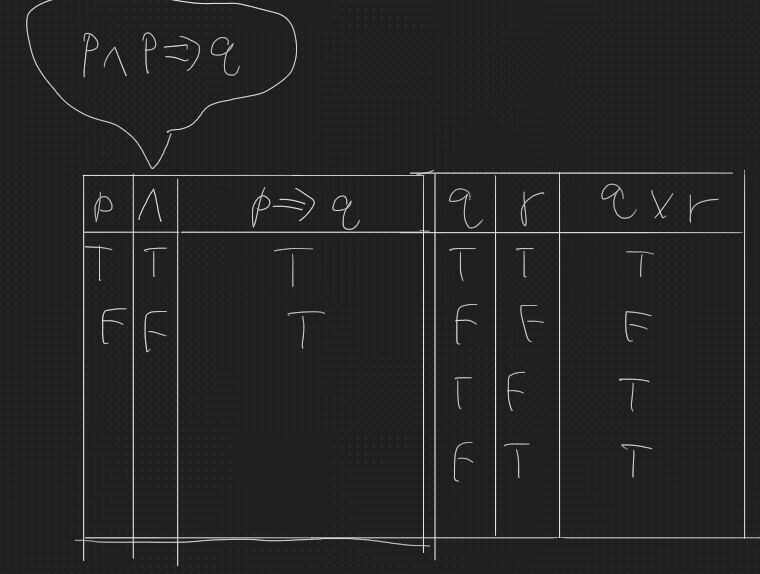
\includegraphics[scale=0.5,]{cap.JPG}
  \end{figure}
  伴意式、$G \models q\lor r$が成立するのは、$(p \wedge (p \Rightarrow q))\Rightarrow q \vee r$がトートロジーのとき、かつその場合のみである。真理値表より、$G$が真である解釈において、$q \vee r$が偽の場合はない。したがって$G \models q\lor r$は成立する。
  \item $G \not\vdash_{r} (q\lor r)$を確認しなさい.
  \item 融合法による反駁証明を用い,
    $G \models q\lor r$が成り立つことを確認しなさい.
  \end{itemize}

\item
  融合法による反駁証明を用いて,
  講義資料「Wumpus Worldにおける推論の例」における
  $(\neg P_{1,2}\land \neg P_{2,1})$を証明しなさい.

\item
  Wumpus Worldにおける風の知覚に関するルール
  「隣の部屋に穴があるとき,またそのときに限り風を感じる」
  と,風の知覚情報$\neg B_{1,1}$, $B_{2,1}$, $\neg B_{1,2}$から,
  場所[3,1]に穴がある$P_{3,1}$ことを証明しなさい.
  %
  ※融合法である必要はありません.各ステップ毎に,利用した推論規則を明示してください.

\item (余力があったらですが..)
  ホーン節を対象とした,前向き推論・後ろ向き推論アルゴリズムを実装してみよう

\end{enumerate}
\end{document}
